\documentclass[11pt]{article}
\usepackage[a4paper,margin=25mm]{geometry}
\usepackage{amsmath,amssymb,amsthm,microtype}
\usepackage{tikz}
\usetikzlibrary{arrows.meta,decorations.markings}
\usepackage{xurl}
\usepackage[hidelinks]{hyperref}
\usepackage{fancyhdr}
\fancypagestyle{draftfirst}{%
 \fancyhf{}
 \renewcommand{\headrulewidth}{0pt}
 \fancyfoot[L]{\small Draft --- 4 November 2026}
 \fancyfoot[C]{\thepage}}
\theoremstyle{definition}
\newtheorem{definition}{Definition}[section]
\newtheorem{example}[definition]{Example}
\theoremstyle{plain}
\newtheorem{proposition}[definition]{Proposition}
\newtheorem{theorem}[definition]{Theorem}
\newcommand{\C}{\mathbb C}
\newcommand{\Z}{\mathbb Z}
\newcommand{\N}{\mathbb N}
\newcommand{\Log}{\operatorname{Log}}
\newcommand{\ev}{\operatorname{ev}}
\newcommand{\state}[3]{s(#1,#2,#3)}
\newcommand{\lean}[1]{\mbox{\texttt{\detokenize{#1}}}}
\hypersetup{pdftitle={A Monodromy Computer by Path Lifting},
 pdfauthor={Xiaoyang Liu}}
\title{A Monodromy Computer by Path Lifting}
\author{Xiaoyang Liu\\[2pt]
 \small University of Waterloo \quad
 \href{mailto:x98liu@uwaterloo.ca}{x98liu@uwaterloo.ca}}
\date{}
\begin{document}
\maketitle
\thispagestyle{draftfirst}
\begin{abstract}
We construct a three-root computer from successive logarithmic lifts
and finite analytic path selection. Five fixed loops yield memory
shifts and conditional writes. A Lean-verified simulation preserves
complete Turing configurations, termination, and divergence.
\end{abstract}

\section{Introduction}

A closed path can return to its base point while changing an analytic
branch. Can this retained change also determine the next operation?

The construction turns winding into a zero-conditional write by
successive logarithmic lifts in one coupled covering, then combines
these operations with finite analytic routing and classical counter
encodings.

\section{Geometric observation}\label{sec:observation}

Write $\C^*=\C\setminus\{0\}$ and $I=[0,1]$.
The exponential covering $\exp:\C\to\C^*$ has fiber
$1+2\pi i\Z$ above $e=\exp(1)$. A fixed based loop and its lift
from $1+2\pi ik$ are
\begin{align}
 b(t)&=\exp(e^{2\pi it}),\label{eq:B}\\
 w_k(t)&=e^{2\pi it}+2\pi ik.\label{eq:circle}
\end{align}
Exponentiation gives~\eqref{eq:B}, and the initial values agree.
The curve $w_0$ winds once around zero. For $k\ne0$, the circle
$w_k$ has radius $1$ and centre at distance $2\pi|k|>1$ from zero,
so its winding number is zero. A second logarithmic lift therefore
changes by $2\pi i$ exactly when $k=0$.

\begin{figure}[!ht]
\centering
\begin{tikzpicture}[x=.65cm,y=.65cm,>=Stealth,font=\normalsize,
 turn/.style={thick,postaction={decorate},
 decoration={markings,mark=at position .18 with {\arrow{Stealth}}}}]
 \draw[->,thin] (-1.8,0)--(2,0);
 \draw[->,thin] (0,-1.25)--(0,7.6);
 \draw[turn] (1,0) arc[start angle=0,end angle=360,radius=1];
 \draw[turn] (1,6.283185) arc[start angle=0,end angle=360,radius=1];
 \draw[fill=white] (0,0) circle[radius=2.5pt];
 \node[below left] at (0,0) {$0$};
 \draw (-.13,6.283185)--(.13,6.283185);
 \node[anchor=east] at (-1.35,6.283185) {$2\pi i$};
 \fill (1,0) circle[radius=1.7pt];
 \node[above right] at (1,0) {$1$};
 \fill (1,6.283185) circle[radius=1.7pt];
 \node[right] at (1,6.283185) {$1+2\pi i$};
 \node[anchor=east] at (-1.35,.7) {$w_0$};
 \node[anchor=east] at (-1.35,7.3) {$w_1$};
 \node at (7.3,0) {$\operatorname{wind}(w_0,0)=1$};
 \node at (7.3,6.283185) {$\operatorname{wind}(w_1,0)=0$};
\end{tikzpicture}
\caption{The lifted circles in the same punctured plane.
They have equal radius and differ by $2\pi i$.
Only $w_0$ surrounds zero, so only its logarithmic lift gains a turn.}
\label{fig:winding}
\end{figure}

\section{The geometric construction}\label{sec:construction}

\subsection*{A shared upper root}
A covering map and a point above the start of a path determine a unique
lift. For analytic coverings, this continues a local inverse branch.
Concatenation composes transport; reversal inverts it; endpoint-fixed
homotopy preserves the returned value \cite[\S1.3]{hatcher}.

To make both lifts admissible, set
$Y=\C\setminus\{0,1\}$ and $D=\exp^{-1}(Y)$.
The restriction $\exp:D\to Y$ is a covering and $0\notin D$.
The loop $b$ lies in $Y$: equality $b(t)=1$ would give
$e^{2\pi it}=2\pi in$ for an integer $n$, contradicting its modulus.
Thus the first lift avoids the puncture required for the second.

The two lower branches should contribute their winding to a shared
upper branch. If $\ell_j$ continues a logarithm along $w_j$, then
\[
 e^{\ell_1+\ell_2}=w_1w_2.
\]
Thus a logarithm of the product accumulates the two logarithmic
increments additively. We use $w_1w_2$ as the common upper input.
To allow an independent upper turn, include a third base coordinate
$v\in\C^*$ and impose
\[
 e^z=v\,w_1w_2.
\]
Solving for the recorded base value $v$ gives the coupled projection
\begin{equation}\label{eq:F}
 F(w_1,w_2,z)=\left(e^{w_1},e^{w_2},\frac{e^z}{w_1w_2}\right)
\end{equation}
from $E=(D\times D)\times\C$ to $X=(Y\times Y)\times\C^*$.
It factors through $L=(D\times D)\times\C^*$ as
\begin{equation}\label{eq:covers}
 E\xrightarrow{\ p\ }L\xrightarrow{\ q\ }X,
\end{equation}
where
\[
 p(w_1,w_2,z)=\left(w_1,w_2,\frac{e^z}{w_1w_2}\right),
 \qquad q(w_1,w_2,v)=(e^{w_1},e^{w_2},v).
\]
The map $q$ is a product covering. The map $p$ is the pullback of
$\exp:\C\to\C^*$ along $(w_1,w_2,v)\mapsto vw_1w_2$, with the
determined coordinate $v$ eliminated.
A state is a retained point of $S=F^{-1}(e,e,1)$.
Put $r_k=1+2\pi ik$. With the principal logarithm, this entire
fiber is uniquely parametrized by
\begin{equation}\label{eq:state}
 \state{k_1}{k_2}{m}
 =\bigl(r_{k_1},r_{k_2},
 \Log r_{k_1}+\Log r_{k_2}+2\pi im\bigr),
 \qquad (k_1,k_2,m)\in\Z^3.
\end{equation}
Indeed, the first two exponential equations give $r_{k_1},r_{k_2}$,
and the third gives precisely the remaining integer $m$.

\begin{definition}[Successive execution]\label{def:execution}
A driver is a triple $\gamma=(u_1,u_2,v)$ of based loops at
$(e,e,1)$ in $X$. From $s=(w_1,w_2,z)\in S$, lift $u_j$ through
the exponential from $w_j$, obtaining $\widetilde w_j(t)$.
Use the resulting path
\begin{equation}\label{eq:feed}
 \eta_s(t)=v(t)\widetilde w_1(t)\widetilde w_2(t)
\end{equation}
as input to an exponential lift from $z$, obtaining
$\widetilde z(t)$. Define $T_\gamma(s)$ to be the three endpoints.
\end{definition}

The lower lifts remain in $D$, so~\eqref{eq:feed} is nonzero.
Its initial value is $w_1w_2=e^z$.
The intermediate curve
$\alpha_s=(\widetilde w_1,\widetilde w_2,v)$ projects by $q$ to
$\gamma$; the complete curve
$\widetilde\gamma_s=(\widetilde w_1,\widetilde w_2,\widetilde z)$
projects by $p$ to $\alpha_s$. Lift uniqueness identifies these
curves with the two covering lifts in Figure~\ref{fig:transport}.
At the final time $e^{\widetilde w_j(1)}=e$ and
$e^{\widetilde z(1)}=\widetilde w_1(1)\widetilde w_2(1)$, since
$v(1)=1$. The endpoint is therefore in the same fiber $S$, ready
to serve as the next initial state.

\begin{figure}[htbp]
\centering
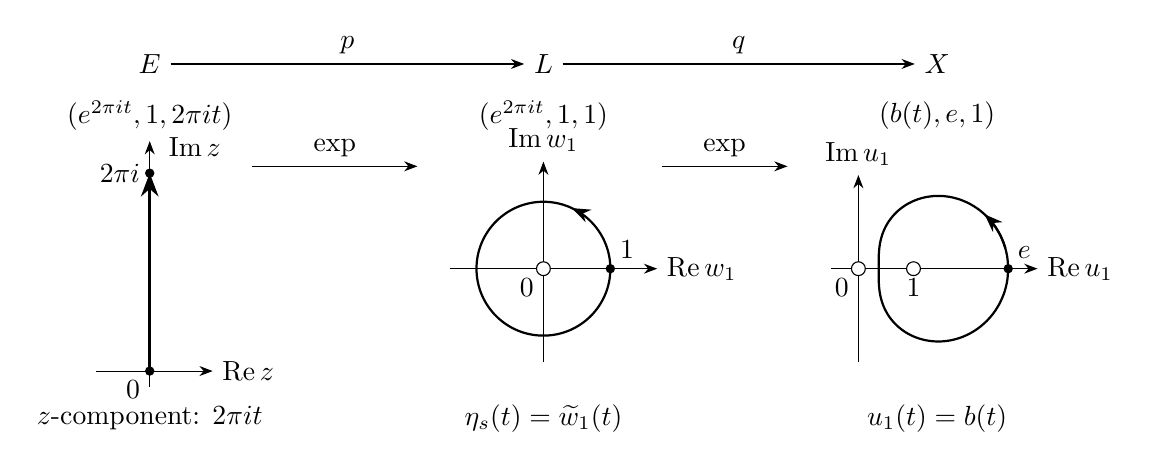
\begin{tikzpicture}[>=Stealth,font=\normalsize,
 turn/.style={thick,postaction={decorate},
 decoration={markings,mark=at position .18 with {\arrow{Stealth}}}}]
 \node (E) at (-5,3.9) {$E$};
 \node (L) at (0,3.9) {$L$};
 \node (X) at (5,3.9) {$X$};
 \draw[->] (E)--node[above] {$p$} (L);
 \draw[->] (L)--node[above] {$q$} (X);
 \node at (-5,3.25) {$(e^{2\pi it},1,2\pi it)$};
 \node at (0,3.25) {$(e^{2\pi it},1,1)$};
 \node at (5,3.25) {$(b(t),e,1)$};
 \draw[->,thin] (-3.7,2.6)--node[above] {$\exp$} (-1.6,2.6);
 \draw[->,thin] (1.5,2.6)--node[above] {$\exp$} (3.1,2.6);
 \begin{scope}[x=.4cm,y=.4cm,xshift=-5cm]
  \draw[->,thin] (-1.7,0)--(2,0);
  \draw[->,thin] (0,-.5)--(0,7.3);
  \draw[very thick,->] (0,0)--(0,6.283185);
  \fill (0,0) circle[radius=1.7pt];
  \fill (0,6.283185) circle[radius=1.7pt];
  \node[below left] at (0,0) {$0$};
  \node[left] at (0,6.283185) {$2\pi i$};
  \node[right] at (2,0) {$\operatorname{Re}z$};
  \node[right] at (.3,7.1) {$\operatorname{Im}z$};
 \end{scope}
 \begin{scope}[x=.85cm,y=.85cm,yshift=1.3cm]
  \draw[->,thin] (-1.4,0)--(1.7,0);
  \draw[->,thin] (0,-1.4)--(0,1.6);
  \draw[turn] (1,0) arc[start angle=0,end angle=360,radius=1];
  \draw[fill=white] (0,0) circle[radius=2.5pt];
  \node[below left] at (0,0) {$0$};
  \fill (1,0) circle[radius=1.7pt];
  \node[above right] at (1,0) {$1$};
  \node[right] at (1.7,0) {$\operatorname{Re}w_1$};
  \node[above] at (0,1.6) {$\operatorname{Im}w_1$};
 \end{scope}
 \begin{scope}[x=.7cm,y=.7cm,xshift=4cm,yshift=1.3cm]
  \draw[->,thin] (-.5,0)--(3.25,0);
  \draw[->,thin] (0,-1.7)--(0,1.7);
  \draw[thick,domain=0:360,samples=80,smooth,variable=\t]
   plot ({exp(cos(\t))*cos((180/pi)*sin(\t))},
         {exp(cos(\t))*sin((180/pi)*sin(\t))});
  \draw[thick,->,domain=8:24,samples=8,smooth,variable=\t]
   plot ({exp(cos(\t))*cos((180/pi)*sin(\t))},
         {exp(cos(\t))*sin((180/pi)*sin(\t))});
  \draw[fill=white] (0,0) circle[radius=2.5pt];
  \draw[fill=white] (1,0) circle[radius=2.5pt];
  \node[below left] at (0,0) {$0$};
  \node[below] at (1,0) {$1$};
  \fill (2.718282,0) circle[radius=1.7pt];
  \node[above right] at (2.718282,0) {$e$};
  \node[right] at (3.25,0) {$\operatorname{Re}u_1$};
  \node[above] at (0,1.7) {$\operatorname{Im}u_1$};
 \end{scope}
 \node at (-5,-.6) {$z$-component: $2\pi it$};
 \node at (0,-.6) {$\eta_s(t)=\widetilde w_1(t)$};
 \node at (5,-.6) {$u_1(t)=b(t)$};
\end{tikzpicture}
\caption{Actual transport for $\gamma=(b,e,1)$ from $s(0,0,0)$.
The tuples are the full curves; the component plots use separate scales.
Read lifting from right to left. The component arrows show
$\exp(\widetilde z)=\eta_s=\widetilde w_1$ and
$\exp(\widetilde w_1)=b$. The right curve is drawn
from $(\operatorname{Re}b,\operatorname{Im}b)
=e^{\cos\theta}(\cos(\sin\theta),\sin(\sin\theta))$, $\theta=2\pi t$.
The upper lift is the straight segment $\widetilde z(t)=2\pi it$.}
\label{fig:transport}
\end{figure}

\subsection*{Five fixed paths}
Besides $b$, take $a(t)=\exp(1+2\pi it)$ and $c(t)=e^{2\pi it}$.
Both $a,b$ are based at $e$ in $Y$; $c$ is based at $1$ in $\C^*$.
Let $A_j$ apply $a$ to coordinate $j$, and $B_j$ apply $b$ there,
with the remaining inputs constant. Let $C$ apply $c$ to the third
base coordinate.

\begin{proposition}[Native operations]\label{prop:gates}
The five actual transports act on the labels~\eqref{eq:state} by
\begin{align*}
 A_1:(k_1,k_2,m)&\longmapsto(k_1+1,k_2,m),&
 A_2:(k_1,k_2,m)&\longmapsto(k_1,k_2+1,m),\\
 B_1:(k_1,k_2,m)&\longmapsto(k_1,k_2,m+[k_1=0]),&
 B_2:(k_1,k_2,m)&\longmapsto(k_1,k_2,m+[k_2=0]),\\
 C:(k_1,k_2,m)&\longmapsto(k_1,k_2,m+1),
\end{align*}
where $[P]$ is $1$ when $P$ holds and $0$ otherwise.
\end{proposition}
\begin{proof}
For $A_j$, the lower lift is $1+2\pi i(k_j+t)$.
Its real part is $1$, so its principal logarithm is continuous.
The upper lift changes by the difference of these logarithms,
preserving $m$. For $B_j$, the lower lift is~\eqref{eq:circle}
and the other memory root is constant. Its winding calculation
gives the conditional upper change. For $C$, both lower roots are
constant and~\eqref{eq:feed} winds once, so the upper lift adds
$2\pi i$. Each displayed trajectory is identified with the actual
lift by uniqueness.
\end{proof}

Products of drivers will be written in execution order.
Concatenation gives $T_{\gamma\delta}=T_\delta\circ T_\gamma$,
and path reversal gives $T_{\gamma^{-1}}=T_\gamma^{-1}$.

\begin{example}[A complete path execution]\label{ex:execution}
Execute the word $A_1B_1B_2A_2^{-1}B_2$ from
$s(-1,1,0)$. The retained complex roots are
\[
\begin{array}{c|ccc}
 \text{completed path}&w_1&w_2&z\\ \hline
 \text{initial}&r_{-1}&r_1&\Log r_{-1}+\Log r_1\\
 A_1&1&r_1&\Log r_1\\
 A_1B_1&1&r_1&\Log r_1+2\pi i\\
 A_1B_1B_2&1&r_1&\Log r_1+2\pi i\\
 A_1B_1B_2A_2^{-1}&1&1&2\pi i\\
 A_1B_1B_2A_2^{-1}B_2&1&1&4\pi i
\end{array}
\]
The first $B_1$ lifts to a circle about zero and writes one upper
turn. The first $B_2$ lifts to a circle centred at $2\pi i$ and
writes none. Reversing $A_2$ brings the second root from $1+2\pi i$
to $1$; the last $B_2$ now writes a turn. Thus the final state is
$s(0,0,2)$. Reversing the word recovers the initial state.
\end{example}

\section{Executable programs}\label{sec:programs}

\subsection*{Selecting the next path}
The conditional operation writes an upper branch. To let this branch
choose the next path, fix $N\ge1$ and put
$\omega_j=e^{2\pi ij/N}$, $0\le j<N$. At a return, observe
\begin{equation}\label{eq:read}
 \rho_N(w_1,w_2,z)=
 \exp\left(\frac{z-\Log w_1-\Log w_2}{N}\right).
\end{equation}
On $S$ it equals $e^{2\pi im/N}$, an $N$th root of $1$.
The logarithms are analytic near every return, since
$\operatorname{Re}w_1=\operatorname{Re}w_2=1$ there.

The normalized divided differences of $u^N$ give the polynomials
\[
 K_j(u)=\frac{u^N-1}{N\omega_j^{N-1}(u-\omega_j)},
 \qquad K_j(\omega_j)=1.
\]
Their values satisfy $K_j(\omega_\ell)=[j=\ell]$.
For a finite driver table $\gamma_j$, set, coordinatewise,
\begin{equation}\label{eq:route}
 \gamma_s(t)=\sum_{j=0}^{N-1}K_j(\rho_N(s))\gamma_j(t).
\end{equation}
The execution language admits~\eqref{eq:read} and~\eqref{eq:route} as
finite analytic observation and path selection at exact fiber returns.
On $S$ they choose one admissible driver; $N$ and the table are fixed
for each program. The routing coefficients stay fixed during the word.
Successive lifting supplies the conditional write; analytic routing
chooses the next word.

\begin{definition}[Finite geometric program]\label{def:program}
A word is a finite concatenation of the five drivers and their
reverses. A program $P$ specifies $N\ge1$, a word $W_j$ and a bit
$h_j$ at each root $\omega_j$. With $\gamma_j$ the driver of $W_j$,
its stopping signal is
\[
 H_P(s)=\sum_jK_j(\rho_N(s))h_j.
\]
If $H_P(s)=1$, execution stops at $s$; otherwise one return executes
$T_{\gamma_s}(s)$. A program return is the completion of the selected
word; its intermediate primitive endpoints do not trigger a new
observation. The complete partial execution $\ev_P(s)$ is the
first stopped state, and is undefined if returns continue indefinitely.
\end{definition}

For example, choose $A_1B_1$ when $\rho_2=1$ and $A_2B_1$ when
$\rho_2=-1$. The successive states
$s(-1,0,0)\mapsto s(0,0,1)\mapsto s(0,1,2)$ show how a conditional
write changes the next selected memory operation. The roots,
the finite table, and lifting determine every return.

\subsection*{Finite control and counters}
Regard the two lower labels as nonnegative counters. A counter
instruction increments counter $i$ and jumps to $q'$, or tests it,
jumping to $q_0$ if zero and otherwise decrementing and jumping to
$q_1$. Include a halt instruction.

\begin{proposition}[Counter realization]\label{prop:counters}
Every finite nonempty two-counter table has a geometric program with the
faithful encoding $(q,n_1,n_2)\mapsto s(n_1,n_2,3q)$.
Each live instruction takes exactly two native returns; halted
instructions stop at their encoded states.
\end{proposition}
\begin{proof}
For $r$ addresses take $N=3r$, reserving phases $3q,3q+1,3q+2$.
An increment executes $C$ first, then $A_iC^{3q'-3q-1}$.
A conditional decrement executes $CB_i$ first. The upper label
becomes $3q+2$ in the zero case and $3q+1$ otherwise.
The next word is respectively $C^{3q_0-3q-2}$ or
$A_i^{-1}C^{3q_1-3q-1}$. Here an integer power of $C$ is the
finite repetition of $C$ or its reverse. Mark phase zero at halt
addresses. Proposition~\ref{prop:gates} verifies these cases;
finite root routing executes their words.
\end{proof}

\section{Turing universality}\label{sec:universality}

The remaining construction translates finite tape computations into
the counter instructions just realized:
\[
 \text{finite tapes}\ \longrightarrow\
 \text{three counters}\ \longrightarrow\
 \text{two counters}\ \longrightarrow\
 \text{geometric words}.
\]
A source machine has finite nonempty control $Q$, finite alphabet
$\Gamma$ with blank $0$, and a partial instruction table
$M:Q\times\Gamma\rightharpoonup
Q\times(\{\mathsf L,\mathsf R\}\sqcup\Gamma)$.
It moves the head or writes a symbol; an absent instruction halts.
A configuration contains control, current symbol, and two
blank-padded half-tapes with finite nonblank support.
Write $\delta_M(c)=c'$ for one instruction step, and call $c$ halted
when no instruction applies. Let $\ev_M(c)$ be the final configuration
when execution halts; it is undefined for an infinite run.

\begin{theorem}[Native geometric Turing universality]\label{thm:universal}
Every such $M$ has a finite geometric program $P_M$, an injective
configuration encoding $\iota_M:\operatorname{Cfg}(M)\to S$, and
a finite root-marked boundary. Its native macro
$\mathcal T_M:S\rightharpoonup S\sqcup\{\mathsf{halt}\}$ reports
$\mathsf{halt}$ when $P_M$'s internal stopping signal is set; otherwise
it executes one native word return by successive lifting, then continues
the same word table until the next marked return. It is defined on
every encoded configuration, with
\begin{align}
 \mathcal T_M(\iota_M(c))&=
 \begin{cases}
  \iota_M(c'),&\text{if }\delta_M(c)=c',\\
  \mathsf{halt},&\text{if }c\text{ is halted}.
 \end{cases}\label{eq:macro}\\
 \ev_{P_M}\circ\iota_M&=\iota_M\circ\ev_M.\label{eq:complete}
\end{align}
Each live source step is a positive finite native first return.
The partial maps in~\eqref{eq:complete} have the same domain: the
configurations from which $M$ halts. Their values encode the same
complete final configuration, so divergence is preserved as well.
Every finite source run is an actual successive lift through
\eqref{eq:covers}, with base paths generated from preceding returned
roots and endpoint the encoded final configuration.
\end{theorem}

\begin{proof}
\emph{Encoding the tape.}
Enumerate $\Gamma=\{0,\ldots,a-1\}$ with blank $0$, and put $B=a+1$.
The canonical half-tape code
$E(d_0d_1\cdots)=\sum_jd_jB^j$ ignores trailing blanks and is
injective: successive remainders and quotients recover every cell.
Pushing a symbol $d$ gives $d+BE$; reading and removing it give
$E\bmod B$ and $\lfloor E/B\rfloor$.
Thus a finite controller storing the pair (control, current symbol),
two counters storing the half-tapes, and a shared workspace counter
can execute every tape instruction. The workspace is zero at each
tape-step boundary.

\emph{Keeping two memory counters.}
To fit the two lower roots, compress these three counters by the
classical prime encoding \cite{minsky}
\[
 (r_0,r_1,r_2)\longmapsto U=2^{r_0}3^{r_1}5^{r_2}.
\]
The second target counter is workspace, again zero at boundaries.
For $(p_0,p_1,p_2)=(2,3,5)$, increment of $r_i$ multiplies by $p_i$;
its test and decrement become divisibility and division by $p_i$.
These are finite counter loops. Multiplication transfers units while
adding $p_i$ for each unit; division counts blocks of $p_i$, keeping
the bounded remainder in finite control. A failed divisibility test
restores the original value. Every such loop terminates and clears
its workspace.

\emph{Executing the encoding.}
Proposition~\ref{prop:counters} compiles the resulting finite table
into geometric words. If $d_M(q,h)$ is the three-counter dispatch
address of $(q,h)$ followed by its two-counter dispatch address, then
\[
 \iota_M(q,L,h,R)=s\bigl(2^{E(L)}3^{E(R)},\,0,\,3d_M(q,h)\bigr).
\]
Injectivity follows from the tape codes, prime encoding, and dispatch
maps. Fixing $M$ fixes the address maps and the finite word table;
$c$ determines only the initial three roots.

\emph{Matching returns.}
Arithmetic loops occupy finite control regions disjoint from the
tape-step dispatches. A second bit table $b_j$ marks precisely
$3d_M(q,h)$; replacing the halt bits $h_j$ by $b_j$ gives a boundary
program with the same words.
A live source step leaves one mark and reaches the next after finitely
many words, with no intervening mark. This proves~\eqref{eq:macro}.
Along these runs, the original halt bits stop exactly at halted
source configurations. Iteration therefore gives~\eqref{eq:complete}:
internal loops introduce neither extra results nor divergence.
Concatenating the selected drivers from their actual returned states
gives the two covering lifts and the encoded endpoint.
The source transition appears in the proof of correspondence; path
generation uses the fixed program and the preceding roots.
\end{proof}

\section{Discussion and verification}

Exponential fibers retain the memory; successive lifting supplies
the conditional write; finite analytic root selection supplies
instruction choice. Classical counter encodings organize these
operations into universal computation. The covering maps and five
primitives are common to all programs; the finite word table and
its root degree depend on the source machine.

Analytic simulation of Turing machines has precedents in Koiran--Moore
\cite{koiran} and Gra\c{c}a--Campagnolo--Buescu \cite{graca}, the
latter including robustness. Cardona et al.\ construct a Turing-complete
stationary Euler flow on a suitably metrized $S^3$ \cite{cardona}.
The present model executes at discrete returns by successive lifting
and finite root selection. A single autonomous flow generating this
execution would require a further construction. The semantics uses
exact fiber states and return tests. Homotopy invariance preserves
transport under admissible based deformations; quantitative error
bounds, physical realization, and computational cost remain separate
questions.

The integrated Lean~4 development verifies the construction and its
simulation chain, using Mathlib's formal computability framework
\cite{carneiro}. Appendix~\ref{app:verification} gives a mathematical
proof index and the commands for reproducing the checks.

\paragraph{AI contributions.}
Generative AI (OpenAI ChatGPT and Codex, including collaborating agents)
contributed substantially to ideation, mathematical constructions,
proofs, Lean formalization, implementation, and manuscript preparation.
The human author directed the research, determined its scope and
principles, critically evaluated the results, and assumes responsibility
for the work. The source accompanies the manuscript for verification.

\begin{thebibliography}{9}\small
\bibitem{hatcher}
A. Hatcher, \emph{Algebraic Topology}, Cambridge University Press, 2002.
\url{https://pi.math.cornell.edu/~hatcher/AT/ATpage.html}.
\bibitem{minsky}
M. L. Minsky, Recursive unsolvability of Post's problem of ``tag'' and
other topics in theory of Turing machines, \emph{Ann. of Math.}
\textbf{74} (1961), 437--455.
\bibitem{koiran}
P. Koiran and C. Moore, Closed-form analytic maps in one and two
dimensions can simulate universal Turing machines,
\emph{Theoret. Comput. Sci.} \textbf{210} (1999), 217--223.
\href{https://doi.org/10.1016/S0304-3975(98)00117-0}{doi:10.1016/S0304-3975(98)00117-0}.
\bibitem{graca}
D. S. Gra\c{c}a, M. L. Campagnolo and J. Buescu, Robust simulations of
Turing machines with analytic maps and flows, in \emph{New Computational
Paradigms}, LNCS \textbf{3526}, Springer, 2005, 169--179.
\href{https://doi.org/10.1007/11494645_21}{doi:10.1007/11494645\_21}.
\bibitem{cardona}
R. Cardona, E. Miranda, D. Peralta-Salas and F. Presas, Constructing
Turing complete Euler flows in dimension 3, \emph{Proc. Natl. Acad.
Sci. USA} \textbf{118} (2021), e2026818118.
\href{https://doi.org/10.1073/pnas.2026818118}{doi:10.1073/pnas.2026818118}.
\bibitem{carneiro}
M. Carneiro, Formalizing computability theory via partial recursive
functions, \emph{ITP 2019}, LIPIcs \textbf{141}, 12:1--12:17.
\href{https://doi.org/10.4230/LIPIcs.ITP.2019.12}{doi:10.4230/LIPIcs.ITP.2019.12}.
\end{thebibliography}

\clearpage
\appendix
\section{Proof index and reproduction}\label{app:verification}
\raggedright

The accompanying Lean~4.35.0 project supplies pinned dependencies.
Its \lean{README.md} records the Git base, exact source fingerprint,
and proof index.
Repository: \url{https://github.com/ERHUTUZI123/monodromy}.

Paths below are relative to \lean{src/Monodromy/}; declaration names
begin with \lean{Monodromy}. Short names retain the preceding namespace.

\paragraph{Conditional winding (Section \ref{sec:observation}).}
A fixed lower loop writes one upper turn precisely on the zero
branch. The actual-lift calculation is
\lean{NestedContinuation.execute_prepare} in \lean{Logarithm.lean}.
The admissible lower covering is
\lean{NestedRestricted.firstCovering}. General transport and homotopy
invariance are established in \lean{Covering.lean}.

\paragraph{The shared fiber and successive execution
(Definition \ref{def:execution}).}
\lean{Continuation.lean} proves that the state fiber has exactly the
labels~\eqref{eq:state}, that both maps in~\eqref{eq:covers} are
coverings, and that the complete runtime curves are their actual lifts.
The principal declarations are
\lean{CoupledContinuation.prepare_surjective},
\lean{prepare_injective},
\lean{CoupledPullback.upperCovering},
\lean{lowerCovering}, and
\lean{CoupledContinuation.restrictedTrajectory_actual_lift}.

\paragraph{Native paths (Proposition \ref{prop:gates},
Example \ref{ex:execution}).}
In \lean{Continuation.lean}, namespace
\lean{CoupledContinuation}, the declarations
\lean{execute_A_left}, \lean{execute_A_right},
\lean{execute_B_left}, \lean{execute_B_right}, and
\lean{execute_control_prepare} give the five return formulas.
The worked word and its reverse are \lean{example_run} and
\lean{example_reverse}.

\paragraph{Internal control (Definition \ref{def:program}).}
The finite-root kernels select a whole prescribed path.
\lean{Choice.lean} and \lean{Radix.lean} establish their analytic
and cardinal properties. Their connection to native execution is
\lean{CoupledContinuation.routeDriver_eq} and
\lean{Program.step_prepare} in \lean{Continuation.lean}.
This is the exact-return domain on which the routed paths are
proved admissible.

\paragraph{Two-counter execution (Proposition \ref{prop:counters}).}
\lean{CounterContinuation.two_returns} in \lean{Counter.lean}
verifies the two-return instruction implementation.
\lean{CounterContinuation.eval_encode} preserves its entire partial
execution. The same file gives the tape and prime-compression
reductions under \lean{Counter.TuringCompiler} and
\lean{Counter.Compression}; canonical tape coding is in
\lean{Tape.lean}.

\paragraph{Native universality (Theorem \ref{thm:universal}).}
\lean{NativeTuring.native_universality} in
\lean{FormalCompilation.lean} combines faithful configuration encoding,
complete partial execution, exact first returns, and finite-run path
realization. Its finite-type forms include
\lean{finiteMacro_iota} and \lean{finite_eval_iota};
\lean{result_actual_lifts} identifies both covering lifts and the
final encoded root. Finite source renaming is in
\lean{FiniteSupport.lean}.

\paragraph{Reproduction.}
From the supplied Lean project root, run
\begin{verbatim}
lake exe cache get
lake build
lake env lean -DautoImplicit=false -DwarningAsError=true src/Audit.lean
\end{verbatim}
The first command obtains the pinned external dependency cache;
the build and audit pass for the supplied source snapshot.
The audit examines every exported Monodromy declaration and its
transitive proof dependencies, allowing only the standard axioms
\lean{propext}, \lean{Classical.choice}, and \lean{Quot.sound}.
\end{document}
